\section{Zielsetzung}
\label{sec:Zielsetzung}
Ziel diese Versuches ist die Anwendung der Tomographie als bildgebendes Verfahren, um die Zusammensetzung verschiedener Würfel zu bestimmen.
Hierbei wird Gammastrahlung verwendet.

\section{Theorie}
\label{sec:Theorie}
In diesem Abschnitt wird die Theorie des Versuchs erklärt, indem zuerst allgemein erklärt wird, was genau die Tomographie ist und wie der Absorptionskoeffizient bestimmt wird.
Anschließend wird die Gammastrahlung betrachtet mit einem besonderem Augenmerk auf dem Zerfall von Caesium und den verschiedenen Wechselwirkungen von Gammastrahlung mit Materie . 

\subsection{Tomographie}
\label{subsec:Tomographie}
Die Tomographie ist ein bildgebendes Verfahren, welches hauptsächlich zur Untersuchung von räumlichen Strukturen benutzt wird, indem mehrere Querschnittsbilder bzw. Projektionen erstellt werden.
Es beruht auf dem Prinzip der Absorption. Dabei wird ein Objekt mit Gammastrahlung bestrahlt und es wird vor und nach der Transmission die Intensität gemessen. Abhängig vom 
Material wird die Intensität unterschiedlich stark absorbiert. Die Materialen besitzen somit verschiedene Absorptionskoeffizienten $\mu_i$.
Nach dem Objekt kann die Intensität
\begin{equation*}
    I = I_0 \text{e}^{-\sum_i \mu_i d_i}
\end{equation*}
bestimmt werden, wobei $I_0$ die Anfangsintensität, $\mu_i$ der Absorptionskoeffizient und $d_i$ die Wegstrecke sind.
Diese Formel kann umgestellt werden zu
\begin{equation}
    \sum_i \mu_i d_i = \text{ln}\biggl(\frac{I_0}{I_j}\biggr),
\end{equation}
welche die Möglichkeit schafft ein Gleichungssystem zu bilden mit dessen Hilfe die Verteilung verschiedener Materialien in einem nicht einsehbaren Körper bestimmt werden kann.
Dafür wird die Messung verschiedener Intensitäten $I_j$ und eine geschickte Auswahl von Strahlwegen benötigt.

\subsection{Gammastrahlung und der Caesium Zerfall}
\label{subsec:GammaCaesium}
In diesem Versuch wird eine Gammaquelle benutzt, weswegen im Folgenden die Gammastrahlung betrachtet wird. Wenn Gammastrahlung auf Matrie trifft entstsehen verschiedene Wechselwirkungen,
welche die Absorption und Abschwächung beeinflussen. 

\subsubsection{Phototeffekt}
\label{subsubsec:Phototeffekt}
Der Phototeffekt tritt eher bei niedrigen Energien auf. Dabei trifft ein Photon auf ein feste Elektron und gibt dabei seine ganze Energie ab. Ist die Phrotoenergie höher als die Bindungsenergie
des Elektron, wird dieses ausgelöst. Das Photoelektron besitzt anschließend die überschüssige Energie des Photons.

\subsubsection{Comptoneffekt}
\label{subsubsec:Comptoneffekt}
Bei dem Comptoneffekt trifft das Photon auf ein kernentferntes Elektron, wobei diese mit einem inelastischen Stoß wechselwirken.
Dabei gibt das Photon nur ein Teil seiner Energie ab und erfährt eine Richtungsänderung und eine Änderung seiner Wellenlänge
\begin{equation}
    \Delta \lambda = \frac{h}{m c} \biggl(1 - \text{cos}(\theta)\biggr).
\end{equation}
Das Elektron erfährt eine Impulsänderung.

\subsubsection{Paarbildung}
\label{subsubsec:Paarbildung}
Die Paarbildung tritt eher bei höheren Energien auf um genau zu sein ab der doppelten Ruheenergie des Elektrons (ca. $\qty{1.02}{\mega\eV}$). Das Photon wird unter Erzeugung eines 
Elektrons und Positrons ausgelöscht. Es wird Energie an den Atomkern abgegeben, aufgrund des Impulserhaltungsatzes. Die Paarerzeugung trägt jedoch nicht zu diesem Versuch bei, weil die 
Energie der Gammastrahlung in diesem Versuch nicht hoch genug ist.

\subsubsection{Caesium Zerfall}
\label{subsubsec:Caesium}
Caesium ist ein Alkalimetall und das Element $\ce{^{137}C}$ zerfällt über einen $\beta^-$-Zerfall in ein metastabiles $\ce{^{137}Ba}$, welches durch Aussendung eines Gammaquants mit einer 
Energie von $\qty{0.662}{\mega\eV}$ in ein stabiles $\ce{^{137}Ba}$ zerfällt. Das Spektrum ist in \autoref{fig:Gammaspektrum} dargestellt, was zeigt, dass das Hauptmaximum bei einer Energie
$\qty{0.662}{\mega\eV}$. Dies ist der Full-Energy-Peak, welcher durch die vollständige Energieabgabe des Photons an das Elektron im Detektor entsteht.

\begin{figure}[H]
    \centering
    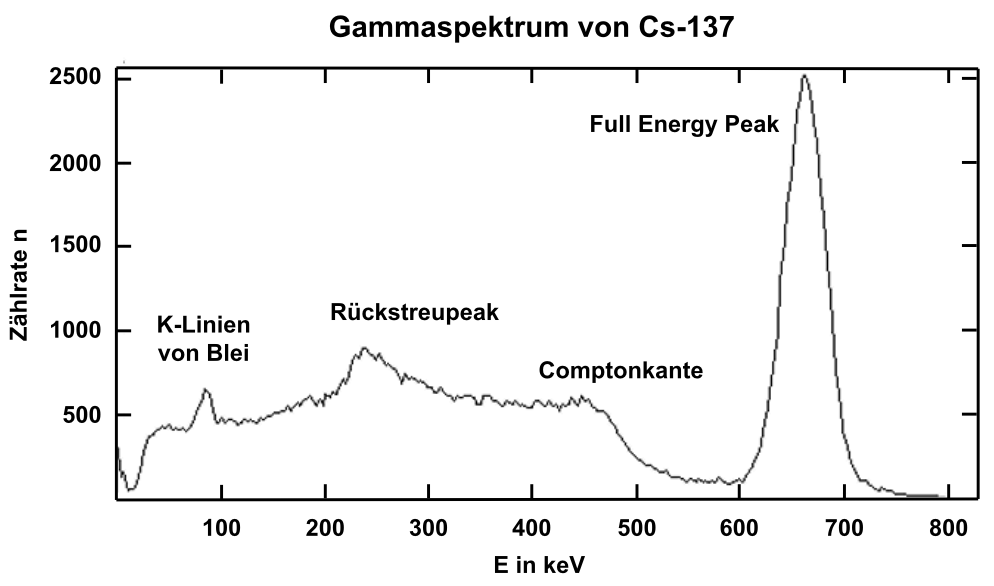
\includegraphics[scale=0.7]{Abbildungen/Gammaspektrum.png}
    \caption{Spektrum der Gammaquelle.\cite{Gammaspektrum}}
    \label{fig:Gammaspektrum}
\end{figure}

Beim Comptoneffekt wird die Energie nur teilweise an das Elektron übertragen. Das Comptonkontinuum, welches sich im linken Bereich der
\autoref{fig:Gammaspektrum} erstreckt, entsteht durch Streuung der Photonen.

\subsection{Messung der Absorptionskoeffizienten}
\label{subsec:Absorptionskoeffizient}



Abschnitte:

Tomographie

Gammastrahlung und Caesium Zerfall

Wechselwirkungen von Gamma Strahlung mit Materie

Berechnung des Schwächungskoeffizienten 



